\section{问题三：FY1 三弹连续投放策略}

问题三将问题二的单弹优化扩展为同一架无人机 FY1 连续投放三枚烟幕弹。与问题二相比，该问的关键变化不是增加三次独立优化，而是要求三枚烟幕弹共享同一无人机航向和飞行速度，并满足相邻投放至少间隔 \(1\,\mathrm{s}\)。因此，若直接把单弹最优方案重复三次，往往会造成遮蔽区间重叠或后续烟幕弹无法进入代表视线附近。

本文 benchmark 沿用目标轴中点代表视线判据，采用固定随机种子的贪心边际覆盖搜索。外层先确定 FY1 的速度与航向，内层逐枚选择投放时刻和引信延迟，使新增烟幕弹对当前未覆盖时间段的边际贡献尽量大。问题三的求解逻辑见图 \ref{fig:q3-model-schematic}。

\begin{figure}[htbp]
  \centering
  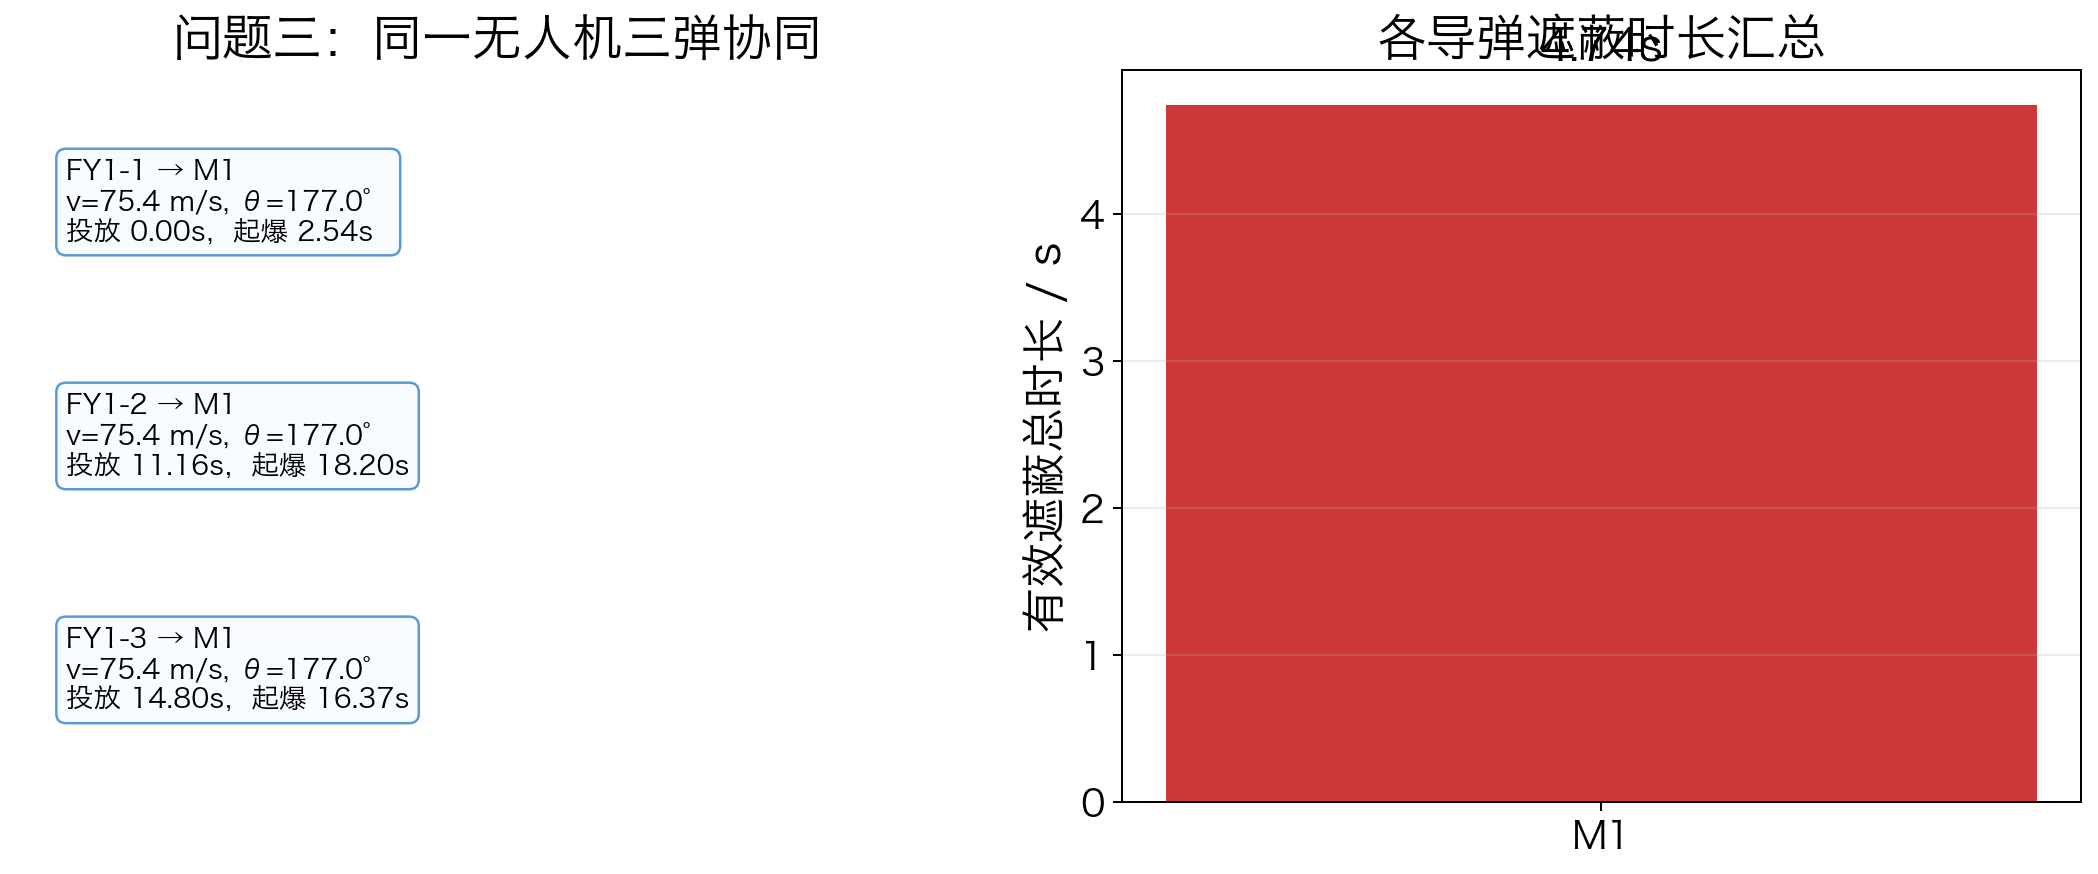
\includegraphics[width=0.94\linewidth]{../figures/fig_q3_model_schematic.png}
  \caption{问题三同一无人机三弹协同示意。三枚弹共用 FY1 的航向和速度，逐枚选择投放与起爆时序。}
  \label{fig:q3-model-schematic}
\end{figure}

搜索得到 FY1 的航向角为 \(177.046501^\circ\)，速度为 \(75.415887\,\mathrm{m/s}\)。三枚弹的投放点、起爆点和单弹有效时长已保存到 \verb|tables/tab_q3_strategy.csv| 和 \verb|tables/result1_benchmark.xlsx|。在当前代表视线判据下，M1 的有效遮蔽区间为 \(2.560000\sim 7.280000\,\mathrm{s}\)，并集遮蔽总时长为 \(4.740000\,\mathrm{s}\)，结果见图 \ref{fig:q3-result}。

\begin{figure}[htbp]
  \centering
  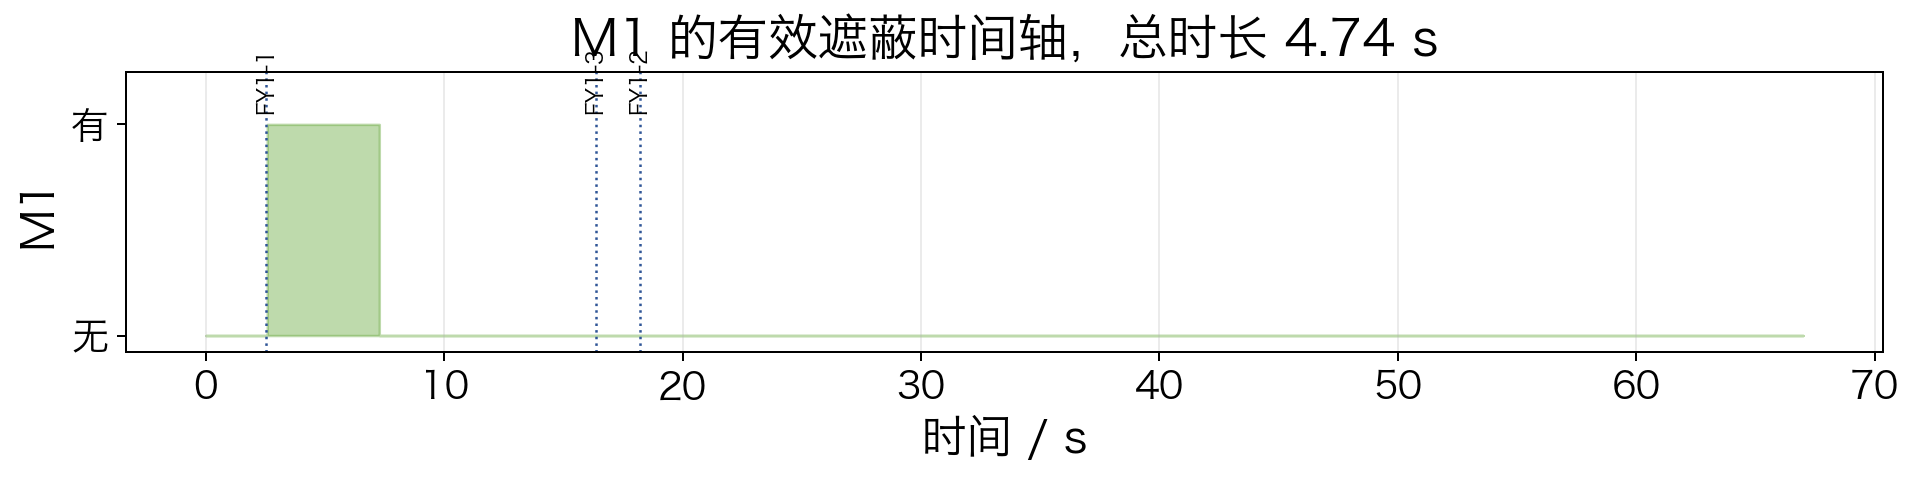
\includegraphics[width=0.92\linewidth]{../figures/fig_q3_result.png}
  \caption{问题三三枚烟幕弹对 M1 的有效遮蔽时间轴。绿色区间表示至少一枚烟幕弹满足代表视线遮蔽判据。}
  \label{fig:q3-result}
\end{figure}

约束检查见图 \ref{fig:q3-validation}。三枚弹的无人机速度均满足 \(70\sim 140\,\mathrm{m/s}\)，起爆高度均为正，投放间隔也满足题设要求。但该结果同时暴露出 benchmark 求解器的不足：第 2、3 枚烟幕弹在当前代表视线判据和贪心搜索策略下没有明显增加并集遮蔽时长。因此本文不把问题三结果表述为最优解，而将其作为后续优化 skill 的反例，用于提醒同航向多弹问题需要真正的联合优化模型。

\begin{figure}[htbp]
  \centering
  
\includegraphics[width=0.92\linewidth]{../figures/fig_q3_validation.png}
  \caption{问题三速度约束和起爆高度检查。该图用于确认策略满足基本物理与题设约束。}
  \label{fig:q3-validation}
\end{figure}
